\documentclass{article}
\usepackage{amsmath, amsfonts, amsthm, amssymb, hyperref, titlesec, graphicx, nameref, titling, caption}
\usepackage[utf8]{inputenc}
\usepackage[margin=2cm,heightrounded=true,centering]{geometry}

\DeclareUnicodeCharacter{2009}{\,}

\titleformat{\section}[block]{\color{black}\Large\bfseries}{}{0em}{}[\rule{\linewidth}{1pt}]
\renewcommand\maketitlehooka{\null\mbox{}\vfill} 
\renewcommand\maketitlehookd{\vfill\null}

\captionsetup[figure]{labelfont={bf},labelformat={default},labelsep=colon,name={Ex}}

\title{\Huge{MATLAB:\\ rand vs. randn}}
\author{\huge{Jacob Lyons}}
\date{\Large 7/16/2021}

\hypersetup{colorlinks=true, linkcolor=blue, filecolor=magenta, urlcolor=cyan,}

\newcounter{ex}[section]
\numberwithin{ex}{section}

\newenvironment{Paragraph}[1][]
{
	{\refstepcounter{ex}}
	\begin{flushleft}
		\textbf{\theex}
	\end{flushleft}
}

\begin{document}
	
	\maketitle
	


	\newpage

\section{Normally Distributed Numbers}

	\large What is the difference between uniformly distributed numbers and normally distributed numbers?
	
	\begin{Paragraph}
		Normal Distribution is a probability distribution which peaks out in the middle and gradually decreases towards both ends of axis.  It is also known as gaussian distribution and bell curve because of its bell like shape.
	\end{Paragraph}
	
	\begin{figure}[h] %%%h,t,p is an option that I’ll explain soon.
		\centering %%%should be clear what this does.
		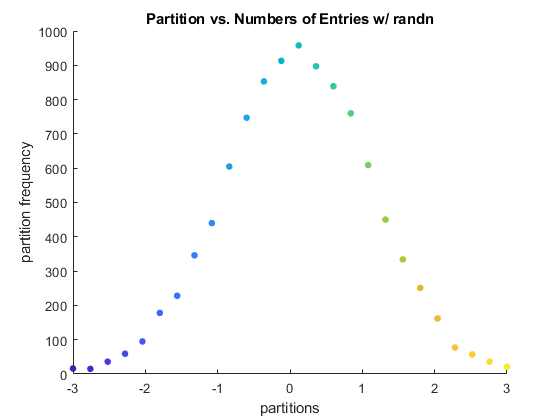
\includegraphics[width=1\textwidth]{randn}
		\caption{\centering Here you can see an example of normal distribution. Notice the bell shape. This was made using randn in MATLAB.}	
	\end{figure} 

	\newpage

\section{Uniformly Distributed Numbers}
	
	\begin{Paragraph}
		Uniform Distribution is a probability distribution where probability of x is constant. That is to say, all points in range are equally likely to occur consequently it looks like a rectangle.
	\end{Paragraph}

	\begin{figure}[h] %%%h,t,p is an option that I’ll explain soon.
		\centering %%%should be clear what this does.
		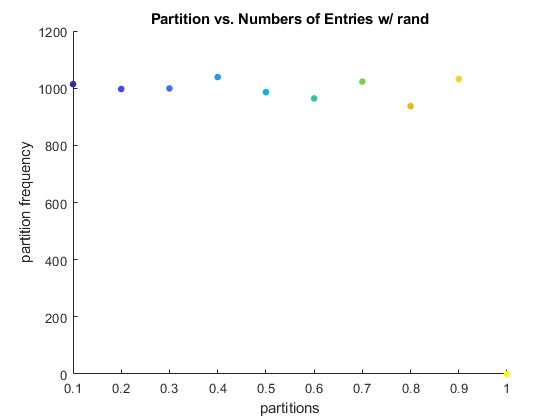
\includegraphics[width=1\textwidth]{rand}
		\caption{\centering Here you can see an example of uniform distribution. Notice the flatter distribution. This was made using rand in MATLAB.}	
	\end{figure} 

\end{document}

